%%==================================================================%%
%% Author : Tejedo Gonz�lez, Daniel                                 %%
%%          S�nchez Barreiro, Pablo                                 %%
%% Version: 1.0, 27/11/2012                                         %%                   
%% Version: 2.0, 09/02/2013                                         %%                   
%%                                                                  %%
%% Memoria del Proyecto Fin de Carrera                              %%
%% Gram�tica,  archivo raiz                                         %%
%%==================================================================%%

\chapterheader{Creaci�n de la gram�tica}{Creaci�n de la gram�tica}
\label{chap:gramatica}

Una vez definida la sintaxis abstracta de nuestro lenguaje, el siguiente paso es definir su sintaxis concreta, que en nuestro caso se trata de una sintaxis textual. Este cap�tulo describe el proceso de desarrollo de una gram�tica que permita definir dicha sintaxis textual.

\chaptertoc

\section{Captura de requisitos}
\label{sec:gram:requisitos}
%%==================================================================%%
%% Author : Tejedo Gonz�lez, Daniel                                 %%
%%          S�nchez Barreiro, Pablo                                 %%
%% Version: 1.0, 27/11/2012                                         %%                   
%%                                                                  %%
%% Memoria del Proyecto Fin de Carrera                              %%
%% Gram�tica,  requisitos                                           %%
%%==================================================================%%

La captura de requisitos de la gram�tica pasa por informarse sobre qu� tipo de sintaxis textual queremos que tengan nuestras operaciones, lo cual en este caso ya estaba especificado previamente por documentos creados en iteraciones previas del proyecto Hydra. Lo m�s l�gico e inmediato era mantenerse fiel a esa sintaxis, seg�n la cual las operaciones deber�an ser expresadas textualmente tal como sigue: \\

Suma: operando1 + operando2

Resta: operando1 - operando2

Multiplicaci�n: operando1 * operando2

Divisi�n: operando1 / operando2

And: operando1 and operando2

Or: operando1 or operando2

Xor: operando1 xor operando2

Implica: operando1 implies operando2

Mayor que: operando1 > operando2

Menor que: operando1 < operando2

Igual que: operando1 == operando2

Mayor o igual que: operando1 >= operando2

Menor o igual que: operando1 <= operando2

Distinto que: operando1 != operando2

Contexto: operando1 [ operando2 ]

Para todo: all operando1 [ operando2 ]

Existe: any operando1 [ operando2 ] \\

Otros aspectos concernientes a la gram�tica que ha habido que tener en cuenta dentro de la fase de captura de requisitos son los siguientes:\\

- Ha de permitirse la posibilidad de especificar prioridad en las operaciones, es decir, de poder delimitar las operaciones con par�ntesis que denoten el orden de realizaci�n de las mismas.

- Todas las representaciones textuales de nuestro lenguaje han de empezar con una l�nea de carga del modelo de caracter�sticas al que han de aplicarse las restricciones. La sintaxis de este aspecto ser� "import operando", donde operando es la direcci�n del fichero hydra del modelo dentro del disco duro del sistema.

- Todas las restricciones definidas han de separarse entre ellas mediante el car�cter '' ; ''.\\

Por supuesto, adem�s de los requisitos aqu� expuestos tambi�n habr� que tener en cuenta todo lo comentado en el apartado de requisitos del cap�tulo anterior, ya que tambi�n influir�n a la hora de tomar decisiones de dise�o en la gram�tica.


\section{Dise�o de la gramatica}
\label{sec:gram:design}
%%==================================================================%%
%% Author : Tejedo Gonz�lez, Daniel                                 %%
%%          S�nchez Barreiro, Pablo                                 %%
%% Version: 1.0, 27/11/2012                                         %%                   %%                                                                  %%
%% Memoria del Proyecto Fin de Carrera                              %%
%% Gram�tica,  dise�o                                       %%
%%==================================================================%%

Una vez han sido definidas las caracter�sticas que queremos que nuestra sintaxis textual posea, el siguiente paso es dise�ar una gram�tica que se ajuste a ellas. 

La parte m�s trivial e inmediata del dise�o de la gram�tica es la concerniente a la implementaci�n de las operaciones, pues las producciones necesarias simplemente requieren la inclusi�n de los operandos involucrados y los caracteres que deseemos que definan la operaci�n. La figura \ref{figopers} muestra la implementaci�n de estas operaciones. 

\begin{figure}[t]
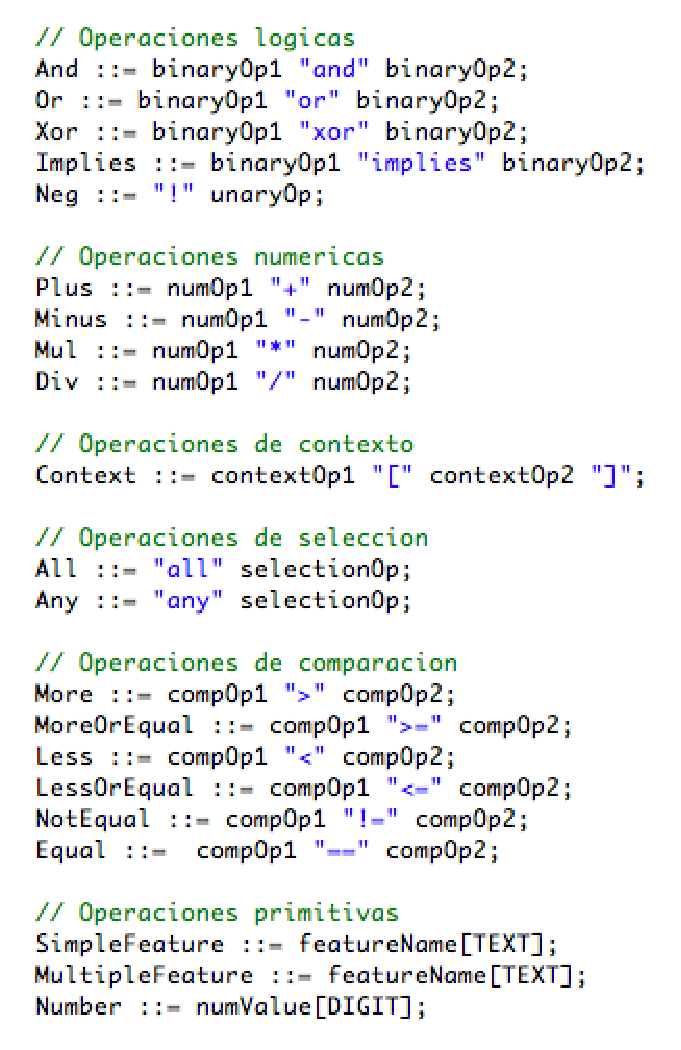
\includegraphics[scale=0.7]{gramatica/operaciones.eps}
\caption{Implementaci�n de las operaciones de nuestro editor com EMFText}
\label{figopers}
\end{figure}

S� que cabe comentar con respecto a las operaciones las �ltimas l�neas, que muestran la asignaci�n de valor a las hojas de nuestros �rboles parseados. En esas l�neas estamos indicando que los atributos de las instancias de clase Number van a ser n�meros, y que los atributos de las instancias de las clases SimpleFeature y MultipleFeature van a ser palabras.

La parte m�s complicada corresponde a la implementaci�n del inicio de la gram�tica y de las producciones que conducen a la misma. Pero antes de mostrar la figura con esta parte de la gram�tica conviene explicar el problema que llev� a realizar los cambios en el metamodelo mencionados en el cap�tulo anterior. Este problema surgi� a la hora de implementar las operaciones con prioridad, es decir, la inclusi�n de los par�ntesis.

El inconveniente es que el tipo de gram�tica LL que implementa EMFText hac�a imposible tomar una decisi�n sobre hacia qu� elemento seguir parseando en caso de encontrarnos con un par�ntesis. La mejor soluci�n que se nos ocurri� para evitar este problema fue la adici�n de diversas clases y relaciones auxiliares en el metamodelo, cuya �nica funci�n es estructural y de apoyo a la gram�tica. Gracias a ellas y a una mejor definici�n de las producciones conseguimos evitar esos problemas de parsing y podemos llevar a cabo las operaciones de prioridad con par�ntesis.

Las clases a�adidas para solventar esta situaci�n fueron las siguientes: BoolPriorityOperand1, BoolPriorityOperand2, NumPriorityOperand1, NumPriorityOperand2, BoolOperandChoices y NumOperandChoices. Las relaciones a�adidas fueron boolPriorityOp1, boolPriorityOp2, numPriorityOp1 y numPriorityOp2.

Una situaci�n similar fue la que propici� que las operaciones Context, All y Any hayan sido dise�adas tal y como presenta el metamodelo, ya que que la particular sintaxis de estas (diferente a las dem�s que siguen el mismo esquema de op + char + op) tambi�n mostraba ciertos problemas de parsing. En este caso no fue necesario a�adir elementos auxiliares, sino simplemente recolocarlos para evitar estos problemas. Con esto ya se han hecho todos los cambios en el metamodelo, que alcanza en este punto su versi�n final tal como muestra la figura \ref{figmetameta}. Con respecto al metamodelo solamente quedan por comentar los m�todos que muestran algunas clases, que ser�n explicados en los pr�ximos cap�tulos ya que se usan en el proceso de validaci�n y sem�ntica.

\begin{figure}[t]
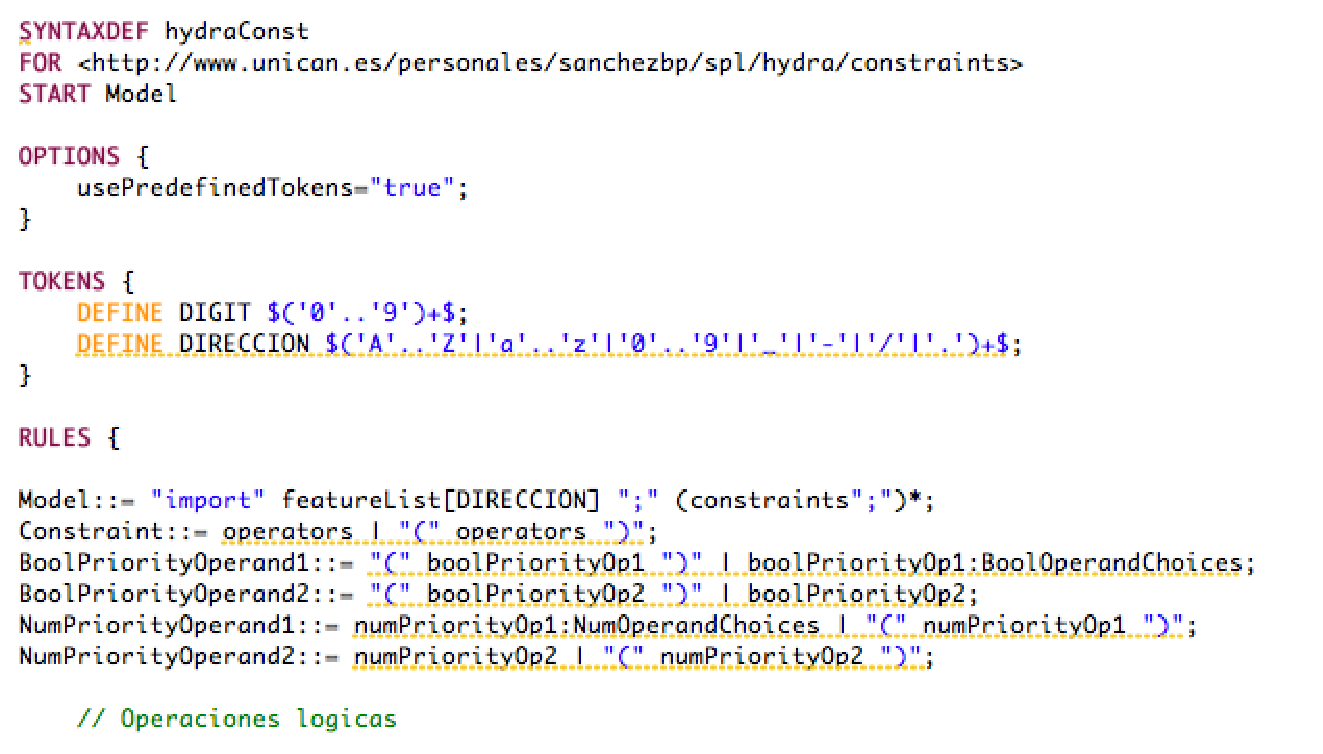
\includegraphics[scale=0.7]{gramatica/iniciogram.eps}
\caption{Implementaci�n del inicio de la gram�tica con EMFText. Con la figura \ref{figopers} se completa la gram�tica}
\label{figinitgram}
\end{figure}

Una vez comentados estos detalles es momento de explicar el inicio de la gram�tica, que se muestra en la figura \ref{figinitgram}. 

En la primera l�nea y mediante la cla�sula SYNTAXDEF indicamos la extensi�n que queremos que tengan los ficheros escritos en nuestro lenguaje. En nuestro caso nos hemos decantado por la terminaci�n .hydraConst. En la segunda l�nea y mediante la cla�sula FOR se indica la URI del metamodelo. Una URI es un formato de direcci�n interno de Eclipse, que se usa para localizar otros ficheros en el workspace. En la tercera l�nea, delimitada por la cla�sula START, indicamos a la gram�tica que la clase inicial de nuestro metamodelo (y la que ser� la raiz en todos los �rboles parseados) es Model.

El bloque OPTIONS permite activar algunas opciones de configuraci�n que incluye EMFText. En nuestro caso la �nica que tiene utilidad es usePredifinedTokens, que permite ahorrarnos la definici�n del token text. El bloque TOKENS sirve para definir los tokens de nuestra gram�tica. En nuestro caso usaremos 3: DIGIT para asignar al valor num�rico, TEXT para asignar a las caracter�sticas y DIRECCION para asignar la direcci�n f�sica del modelo de caracter�sticas.

Por �ltimo, el bloque RULES permite crear las producciones. Como inicial, tal y como se especific� en los requisitos, exigimos un import y una direcci�n, que ser� almacenada en el atributo featureList de la clase Model. En la l�nea inicial tambi�n se indica, mediante una expresi�n regular, que el n�mero de restricciones a definir puede ser tan grande como se desee y que estas deben acabar con el car�cter '';'' .

La l�nea de producci�n de Constraint diferencia entre operaciones con prioridad y sin ella. Sin el problema comentado de EMFText la gram�tica podr�a quedar as�, pero para solucionarlo nos vemos obligado a incluir las cuatro l�neas siguientes, cuya �nica funci�n es solventar esa situaci�n. El resto de la gram�tica continuar�a en la figura \ref{figopers} mostrada anteriormente, y ah� terminar�a.






\section{Pruebas}
\label{sec:gram:pruebas}
%%==========================================================================%%
%% Author : Abascal Fern�ndez, Patricia                                     %%
%% Author : S�nchez Barreiro, Pablo                                         %%
%% Version: 1.4, 29/04/2013                                                 %%
%%                                                                          %%
%% Memoria del Proyecto Fin de Carrera                                      %%
%% Domain Engineering/Pruebas con EUnit                                     %%
%%==========================================================================%%
EUnit es un sistema de pruebas \cite{kolovos:2008} unitarias que proporciona assertions para la comparaci�n de modelos, archivos y directorios. Una \emph{assertion} es un predicado, verdadero o falso, colocado en un programa para indicar que el desarrollador cree que el predicado es siempre cierto en ese lugar. Las pruebas pueden reutilizarse con diferentes conjuntos de modelos y datos de entrada, y las diferencias entre los modelos esperados y los reales pueden ser visualizadas gr�ficamente.

Al comenzar la fase de pruebas me encontr� con el problema inicial de que EUnit no ten�a implementada la comparaci�n de fragmentos de texto en los ficheros generados que era precisamente la manera de comprobar que los generadores de c�digo funcionaban correctamente. De tal forma proced� a realizar una petici�n en el foro de la plataforma e incorporaron una nueva assertion denominada \imp{assertLineWithMatch} que permit�a comprobar si un fichero dispon�a de un determinado fragmento de texto o no (l�neas 1-4 del listing \ref{dom:code:eunit}). Tambi�n era necesario comprobar que los ficheros y directorios se creaban correctamente por lo que la assertion \imp{assertEqualDirectories} es v�lida para tal fin (l�neas 6-9 del listing \ref{dom:code:eunit}). Y por �ltimo, se debe comprobar que las plantillas lanzan las excepciones oportunas para los casos no v�lidos, mediante la combinaci�n de las instrucciones \imp{assertError} y \imp{runTarget}, se puede comprobar si el fichero deseado lanza o no una excepci�n (l�neas 11-16 del listing \ref{dom:code:eunit}). Con estas assertions se procede a realizar todos los casos de prueba descritos en la tabla \ref{dom:table:bid} con resultados satisfactorios.

\begin{lstlisting} [basicstyle=\ttfamily\scriptsize,language=CSharp, captionpos=b,
                    caption=Pruebas de los generadores de c�digo con EUnit,
                    label=dom:code:eunit]
01 @test
02 operation classWithNameAndWithoutType() {
03    assertLineWithMatch(path+"Data\\src\\BasicGraph\\Edge.cs",
                          "partial class Edge");
04 }
05 ...
06 @test
07 operation emptyPackage() {
08    assertEqualDirectories(path+"Data\\src\\PaqueteVacio",
                             path+"\\Data\\src\\PaqueteVacio");
09 }
10 ...
11 @test
12 operation thowsExceptions() {
13    ...
14    assertError(runTarget(pathTemplates+'\\ParametersCreation.egl'));
15    ...
16 }
\end{lstlisting}


\begin{table}%
\begin{tabularx}{17cm}{|l|X|l|}
 \hline
{}&{Casos v�lidos}&{Casos no v�lidos} \\ \hline
\multirow{12}{*}{Clase} & Clase con nombre. & Clase fuera de un paquete. \\
& Clase tipo abstract. & Clase sin nombre.\\
& Clase sin tipo. & Clase enumerada.\\
& Clase que hereda de una o varias clases. &\\
& Clase que hereda de una o varias interfaces. &\\
& Clase que hereda de clases e interfaces. &\\
& Clase sin propiedades. &\\
& Clase sin m�todos. &\\
& Clase sin propiedades ni m�todos. &\\
& Clase con propiedades. &\\
& Clase con m�todos. &\\
& Clase con propiedades y m�todos. &\\
\hline
\multirow{4}{*}{Paquete} & Paquete con nombre. & Paquete sin nombre. \\
& Paquete con clases e interfaces en su interior. & \\
& Paquete vac�o. & \\
& Paquete dentro de otro paquete (recursividad). & \\
\hline
\multirow{4}{*}{Clase Enumerada} & Clase enumerada con nombre. & Clase enumerada sin nombre. \\
& Clase enumerada con literales. & \\
& Clase enumerada vac�a. & \\ 
\hline
\multirow{3}{*}{Interfaz} & Interfaz con nombre. & Interfaz sin nombre. \\
& Interfaz sin m�todos. & Interfaz fuera de paquete.\\
& Interfaz con m�todos. & \\
\hline
\multirow{10}{*}{Propiedad} & Propiedad con nombre. & Propiedad sin tipo. \\
& Propiedad sin nombre (se debe poner uno por defecto). & Asociaciones sin multiplicidad.\\
& Propiedad est�tica (no lleva m�todos getter ni setter). & \\
& Propiedad protected (no lleva m�todos getter ni setter). & \\
& Propiedad no est�tica (lleva m�todos getter ni setter). & \\
& Propiedad es una colecci�n. & \\
& Propiedad es una asociaci�n simple. & \\
& Propiedad es una asociaci�n bidireccional one to one. & \\
& Propiedad es una asociaci�n bidireccional one to many. & \\
& Propiedad es una asociaci�n bidireccional many to many. & \\
\hline
\multirow{14}{*}{M�todo} & M�todo con nombre. & \\
& M�todo sin nombre (se debe poner uno por defecto). &  \\
& M�todo sin tipo (se debe poner void por defecto). &  \\
& M�todo sin tipo (se debe poner void por defecto) y sin par�metros. & \\
& M�todo sin tipo (se debe poner void por defecto) y con par�metros. &  \\
& M�todo void sin par�metros. &  \\
& M�todo void con par�metros. &  \\
& M�todo retorna tipo primitivo sin par�metros. &  \\
& M�todo retorna tipo primitivo con par�metros. &  \\
& M�todo retorna colecci�n sin par�metros. &  \\
& M�todo retorna colecci�n con par�metros. &  \\
& M�todo est�tico. &  \\
& M�todo abstracto. &  \\
& M�todo protected. &  \\
\hline
\multirow{3}{*}{Par�metros de m�todo} & Par�metro con nombre. & Par�metro sin tipo. \\
& Par�metro sin nombre (se debe poner uno por defecto). & \\
& Par�metro con tipo. & \\
\hline
\multirow{2}{*}{Herencia} & Herencia simple. &   \\
& Herencia m�ltiple (se debe implementar interfaces y clases adicionales, si fuera necesario). & \\
\hline
\end{tabularx}
\caption{Soluci�n para evitar incoherencias en el c�digo C\# en la bidireccionalidad one to one}
\label{dom:table:bid}
\end{table}%

Durante este cap�tulo se han descrito la fase de \emph{Ingenier�a del Dominio} de nuestra l�nea de productos software. Dentro de dicha fase se ha analizado c�mo se transforman los elementos del modelo a c�digo C\#, el desarrollo e implementaci�n de los generadores de c�digo junto con la explicaci�n de varios ejemplos y se ha conclu�do con la fase de pruebas.


